\section{What is WebRTC?}

%% 
%% Leave first page empty
\thispagestyle{empty}

Web Real-Time Communication is an standard that will help to build P2P applications in the developer layer relying in a defined API. The first announcement went public in a working group of the World Wide Web Consortium (W3C) in May 2011 \cite{webrtcW3cgroup} and started the official mailing list in April 2011 \cite{welcomeW3C}. During the first stage of discussion, the main goal was to define a public draft for the API implementation and a route timeline with the goal to standardize the protocol by ends of 2012. The first public draft of W3C came public the 27th of October 2011 \cite{originalW3Cdraft}. During this first W3C draft, only media (audio and video) could be sent over the network to other peers, they focused in the way browsers will be able to access the media devices without using any plugin or external software.

Alongside to the W3C working group, the WebRTC concept also joined the IETF with a Working Group (WG) in May 2011 \cite{webrtcIETFgroup} with the first public announcement charter done the 3th of May 2011 \cite{webrtcIETFcharter}. The milestones of the WG initially marked December of 2011 as deadline to provide the information and elements required to the W3C for the API design input. On the other side, the main goals of the WG covered the definition of the communication model, session management, security, NAT traversal solution, media formats, codec agreement and transport of the data \cite{webrtcIETFcharter}. All goals have evolved during the standardization process with the work done along with the W3C WG.

One  of the most important steps during the process of standardization came the 1st of June 2011 when Google publicly released the source code of their API implementation \cite{haraldpublicWebRTC}. 

During all this period both WGs have been working alongside to provide a reliable solution to enable applications to perform media and data peer-to-peer transfer in a plugin-free environment. The first final version of the WebRTC API is to be published during March 2013.

\subsection{Support}

The following companies have supported and are actively working in the development of WebRTC standard in the W3C: Google, Mozilla and Opera \cite{googleAnnouncement}. Other companies such as Microsoft have supported browser-to-browser solution but have published their own proposal which differs with the one published in the WebRTC WG, called CU-RTC-Web \cite{curtcweb}, this proposal did not get much traction by the workgroup being declined to unify with the current specs, during an W3C workgroup poll in September 2012 the chairs of the group decided to attach to the already existing WebRTC API instead of moving it to the CU-RTC-Web \cite{curtcpoll}.

During the firsts attempts to build a reliable solution for WebRTC Ericsson Labs presented an initial API based on the preliminary work done in the WHATWG, this API was called ConnectionPeer API and required an special module to be installed in your browser \cite{ericssonwebrtc}. Ericsson lately dropped from the effort to build it's own browser to focus in the standardization and codec discussion, leaving the API implementation to the Mozilla and Chrome teams. The original API evolved rapidly during the next months thanks to the WGs and the developer community feedback that is experimenting with the unstable API.

\subsection{Milestones}

During the process of standardization some important moments should be remarked. In January 2012 Opera implemented the first version of WebRTC getUserMedia for accessing the camera and audio \cite{operaannouncement}, during this year getUserMedia is available in the stable version of Opera. 

Google Chrome integrated the first version of WebRTC in its DEV and Canary channels of the browser during January 2012 \cite{chromeannouncement}, in June 2012 it started moving its API to the stable channel hidden behind a flag, in November 2012 WebRTC becomes fully available in Google Chrome stable channel and is open for public usage \cite{chromestable}. 

Mozilla Firefox started working on the getUserMedia implementation early 2012 delivering the first version of media access trough API at the beginning of 2012 in the alpha version \cite{mozillablog}, in April 2012 Mozilla published a WebRTC video demo running on Firefox in the "adler" channel \cite{mozillawebrtc}, also supporting some primitive DataChannel API. Later in October Firefox Nightly was carrying the first unstable version of the WebRTC API including DataChannel \cite{mozillafinal}, Mozilla announced in September 2012 that the stable version of WebRTC will be shipped along with Firefox 18 in January 2013 \cite{mozillacomming}. 

Some announcements done from Microsoft point out that they are also working in some implementation into Internet Explorer by using CU-RTC-Web as the default standard, at the moment only the Media API information is publicly available \cite{microsoftcapture}.

Some mobile platform important moments should be pointed out. In October 2012 Ericsson announced the world's first WebRTC-enabled browser for mobile devices called "Bowser" with support for iOS and Android, this browser is able to handle WebRTC calls using RTCWeb Offer/Answer Protocol (ROAP) which is an old discontinued version of the WebRTC API that has moved to Javascript Session Establishment Protocol (JSEP). This browser also differs from the previous desktop alternatives on the codec side, it is carrying H.264 for video and G.711 for audio \cite{ericssonbowser}. The API provided by Bowser is not fully W3C compliant.

\subsection{WebRTC architecture}

How WebRTC works, simple topology and key points.

\subsection{Alternatives}

Some alternatives are available to the WebRTC concept, considering the global architecture of WebRTC, Session Initiation Protocol (SIP) and Secure Real-Time Media Flow Protocol (RTMFP) are similar approaches to the same solution.

\subsubsection{SIP}

Both SIP and RTMFP are protocols to allow communication between two different users with audio/video support. SIP is an open standard and RTMFP is a proprietary protocol by Adobe, both systems are widely used for real-time communication. SIP final Request for Comments (RFC) was published in June 2004 \cite{sipRFC}, this document describes the methods and behaviors of SIP. From an overview perspective, SIP is an application-layer control protocol for multimedia sessions, can establish, maintain and terminate them, during the development of the standard different new functionalities were added to the drafts such as conferencing and the possibility of adding/removing media from existing sessions. SIP differentiates from RTMFP/WebRTC by locating the end user to be used for communication, this feature allows SIP to be closely related to traditional PSTN networks as it allow cross-domain communication which is not possible when using RTMFP/WebRTC. SIP is not a complete toolkit for communications, it works alongside with other existing protocols such as Real-time Transport Protocol (RTP), Real-Time Streaming Protocol (RSTP), Session Description Protocol (SDP) and Media Gateway Control Protocol (MEGACO). Using SDP for the session negotiation between the end-points and RTP/RSTP for the media transport, all those protocols usage is widely extended in the network and provides legacy for older technologies. Meanwhile SIP can locate and deliver a message to a user, SDP can provide the required information for the session establishment and RTP can transport the media specified in the SDP body.

\begin{figure}[h]
  \centering
    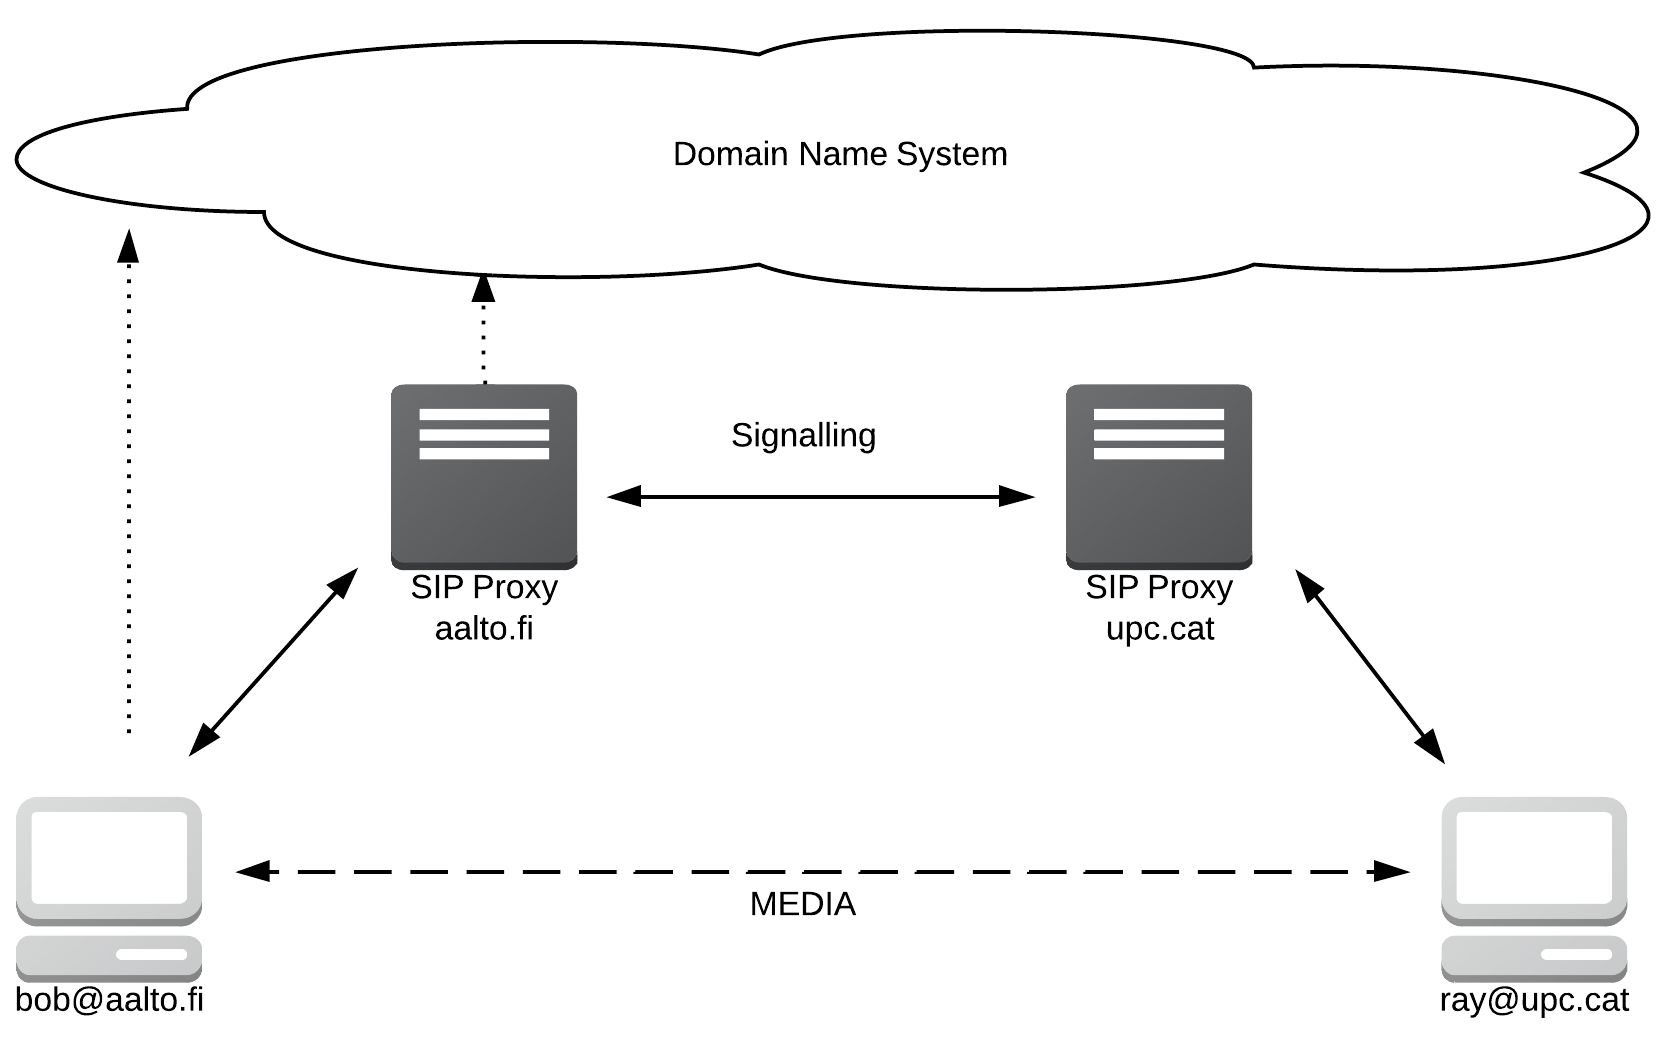
\includegraphics[width=1\textwidth]{./figures/SIParchitecture.png}
      \caption[SIP architecture for end-to-end signaling]{SIP architecture for end-to-end signaling.}
	\label{fig:SIParchitecture}
\end{figure}

SIP architecture relies in a trapezoid form where the Domain Name System (DNS) is used to locate the other peers of the system, once that peer is located and session is negotiated, media flows peer-to-peer directly to the endpoint. In order to build this system different agents are needed, SIP Proxies, SIP Redirect and SIP Registrar. SIP Proxies transmit the SDP and SIP messages from one peer to the other to establish communication (Figure ~\ref{fig:SIParchitecture}). SIP Registrar are the machines that collect and save all the user information from the end points.

DNS provides the IP address for both proxy servers and allow the messages to be exchanged between both peers, when SIP is used the following messages are exchanged: INVITE, RINGING and 200OK. Those messages carry the SDP data inside in an object format, when ray@upc.cat receives the INVITE message from bob@aalto.fi builds the 200OK response carrying the SDP object that providing compatibility check between both peers and which options and codecs to use. SIP provides some more messages to update the already existing session or to close them. The media transport is done using RTP and RTCP that rely over User Datagram Protocol (UDP), for Network Address Translation (NAT) SIP uses other protocols such as Session Traversal Utilities for NAT (STUN) \cite{sipRFC}.


Talk about SIP, RTMFP and WebRTC.



\subsection{Issues in WebRTC}

WebRTC uses a mixture of different technologies to perform peer-to-peer communication between clients, those technologies range from SRTP, RTP, RTCP and multiple codecs that are being discussed. This scenario makes performance the key point for success in developing stable WebRTC applications. 

Performance is manly related to computer capabilities and the ability to encode/decode at the same time as transferring and monitoring multiple peer connections. All those tasks are run over the browser and not directly on the OS, this is good for interoperability between platforms but bad in the performance aspect. 

Media applications are delay sensitive and require a low packet loss for its proper function, WebRTC is working on this aspect by trying to implement congestion control over the connection stablished between peers, this work has not been completed yet and will arise as a problem in the near future. Packet loss due to system capacity and bandwidth are measurable in WebRTC using the Stats API, this API provides information about the PeerConnection performance and is accessible by JavaScript.

Constraints and bandwidth statistics will make a big difference in how media is acquired in WebRTC. Browsers and web applications have always tolerate some amount of delay and packet losses but this is not possible in media infrastructures for real time conversations, a change of scope is needed to handle Quality of Service (QoS) in WebRTC.

